\chapter{Beispiele}\label{beispiel}

Beispielkapitel.
\lipsum[2]

\section{Ein Abschnitt}
Beispielabschnitt.

Aufzählungen werden mit der \code{enumerate} Umgebung erstellt:
\begin{enumerate}
  \item{Beispielpunkt A}
  \item{Beispielpunkt B}
  \item{\ldots}
\end{enumerate}

Sollen nur Stichpunkte abgebildet werden, so nimmt man dafür eine \code{itemize} Umgebung:
\begin{itemize}
  \item{Beispielpunkt C}
  \item{Beispielpunkt D}
  \item{\ldots}
\end{itemize}

\subsection{Ein Unterabschnitt}

Beispieltext.

\subsubsection{Ein Unter-Unterabschnitt}

Das ist die niedrigste Ebene.

\section{Tabellen}

Tabelle~\ref{tab:bsp} ist eine Beispieltabelle.
Man beachte die Position der Beschriftung.
\lipsum[1]

\begin{table}[!htbp]
  \caption{Beispieltabelle}\label{tab:bsp}
  \centering{%
    \begin{tabular}{|c|c|}
      \hline
      \textbf{Zeitpunkt (s)} & \textbf{Wert} \\
      \hlineB{3}
      0                      & 0.0           \\
      \hline
      1                      & 0.3           \\
      \hline
      2                      & 0.9           \\
      \hline
    \end{tabular}
  }
\end{table}

Ein wenig aufwendiger ist Tabelle \ref{tab:bsp2}.
\lipsum[3]

\begin{table}[!htbp]
  \caption{Tabelle mit \code{tabularx}, farbigen Zellen und Multicolumn.}
  \label{tab:bsp2}
  \centering {
    \sffamily
    \begin{tabularx}{0.3\textwidth}{|X|l|}
      \hline
      \rowcolor{gray!30!white}\multicolumn{2}{|c|}{\textbf{Schema} EAV} \\
      \hline
      \rowcolor{gray!30!white}\textbf{Spalte} & \textbf{Datentyp}       \\
      \hline
      \underline{id}                          & INTEGER                 \\
      \hline
      entität                                 & VARCHAR                 \\
      \hline
      attribut                                & VARCHAR                 \\
      \hline
      wert                                    & FLOAT                   \\
      \hline
    \end{tabularx}
  }
\end{table}

\section{Grafiken}

\lipsum[1]

\subsection{Rastergrafik}

Bild~\ref{fig:bsp} zeigt das Hochschullogo.
Es wird als JPEG-Datei eingebunden.
Man kann aber auch andere Formate wie PNG, EPS oder PDF auf diese Weise einbinden.

\begin{figure}[!htbp]
  \centering{%
    
\includegraphics[width=0.2\linewidth]{bilder/HSLogo.jpg}
    \caption{Logo der Hochschule Wismar}\label{fig:bsp}
  }
\end{figure}

\lipsum[2]

\subsection{In \LaTeX{} erzeugte Grafiken}

Bild~\ref{fig:tikzbsp} erzeugt eine Grafik mit dem Paket Ti\textit{k}Z\index{Ti\textit{k}Z}.

\begin{figure}[!htbp]
  \centering{%
    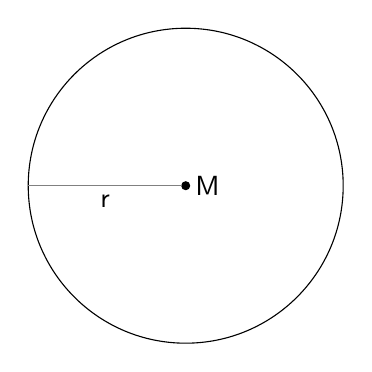
\begin{tikzpicture}
      \draw[black, thin] (0,0) circle (2);
      \filldraw[black] (0,0) circle (0.05) node[right] {\sffamily{M}};
      \draw[gray, thin] (-0.05,0) -- (-2,0) node[black, below, pos=0.5] {\sffamily{r}};
      \end{tikzpicture}
      \caption{Grafik mit Ti\textit{k}Z}\label{fig:tikzbsp}
  }
\end{figure}

So können beispielsweise auch Schaltpläne direkt im \LaTeX-Quelltext skizziert werden, wie Bild \ref{circuit} zeigt.

\begin{figure}[!htbp]
  \centering{%
    \begin{tikzpicture}[scale=0.5, circuit ee IEC, font=\sffamily\footnotesize]
      \tikzset{%
        Pfeil/.style={thick,shorten >=#1,shorten <=#1,->,>=latex},
        UPfeil/.style={blue,Pfeil=#1,font={\sffamily\itshape}},
        IPfeil/.style={red,Pfeil=#1,font={\ttfamily\itshape}}
      }

      \draw (0,0) -- (2,0)
      (3,3) -- (3,5)
      (3,-3) -- (3,-5)
      (2,-3) -- (2,3)
      (4,-3) -- (4,3)
      (2,3) -- (4,3)
      (2,-3) -- (4,-3)
      (2,1) -- (4,1)
      (2,-1) -- (4,-1)
      (8,-5) -- (8,5)
      (6,0) -- (8,0)
      (10,0) -- (12,0)
      (12,2) -- (12,-2)
      (13,2) -- (12,1)
      (13,-2) -- node [rotate=-45]{$\blacktriangleright$} (12,-1)
      (13,2) -- (13,5)
      (13,-2) -- (13,-5);

      \draw[fill=white] (0,0) circle (4pt) node [left] {$B^+$}
      (3,5) circle (4pt) node [left] {$C^{++}$}
      (3,-5) circle (4pt) node [left] {$E^0$}
      (6,0) circle (4pt) node [left] {$B^+$}
      (8,5) circle (4pt) node [left] {$C^{++}$}
      (8,-5) circle (4pt) node [left] {$E^0$}
      (10,0) circle (4pt) node [left] {$B^+$}
      (13,5) circle (4pt) node [left] {$C^{++}$}
      (13,-5) circle (4pt) node [left] {$E^0$};

      \draw[fill=black] (8,0) circle (4pt);

      \node [diode={circuit symbol size = width 8pt height 8pt}, point down] at (8,-2) {};
      \node [diode={circuit symbol size = width 8pt height 8pt}, point up] at (8,2) {};

      \draw[dashed] (4,3) -- (7,3)
      (4,1) -- (7,1)
      (4,-1) -- (7,-1)
      (4,-3) -- (7,-3);

      \node at (3,2) {$n$};
      \node at (3,0) {$p$};
      \node at (3,-2) {$n$};

      \draw[IPfeil=0em](12.5,-2.5) -- node [left]{$I_E$}(12.5,-4);
      \draw[IPfeil=0em](12.5,4) -- node [left]{$I_C$}(12.5,2.5);
      \draw[IPfeil=0em](10,0.5) -- node [above]{$I_B$}(11.5,0.5);
      \draw[UPfeil=0em](10,-0.5) -- node [right, yshift=1em]{$U_{BE}$}(10,-4.5);
      \draw[UPfeil=0em](13.5,4.5) -- node [right]{$U_C$}(13.5,2.5);
      \draw[UPfeil=0em](15,4.5) -- node [right]{$U_{CE}$}(15,-4.5);
    \end{tikzpicture}
    \caption{Beispiel für einen Schaltplan mit Ti\textit{k}Z}
    \label{circuit}
  }
\end{figure}

Das Paket \code{smartdiagram} bietet darüber hinaus auch Funktionen zur automatischen Erzeugung spezieller Grafiken (siehe Bild \ref{fig:smart}).
Mehr dazu in der entsprechenden Dokumentation \cite{smart}.

\begin{figure}[!htbp]
  \centering{\smartdiagram[sequence diagram]{Rühren,Kneten,Backen}}
  \caption{Sequenzdiagramm mit dem \code{smartdiagram} Paket}
  \label{fig:smart}
\end{figure}

Natürlich können Plots und andere Grafiken in den Programmen der Wahl erstellt und dann als Bilddatei mit einem \verb$\includegraphics$ eingebunden werden.
Allerdings ist auch dies in \LaTeX{} direkt möglich, wie Bild \ref{fig:plot} zeigt\index{Plot}.

\begin{figure}[!htbp]
  \center {
    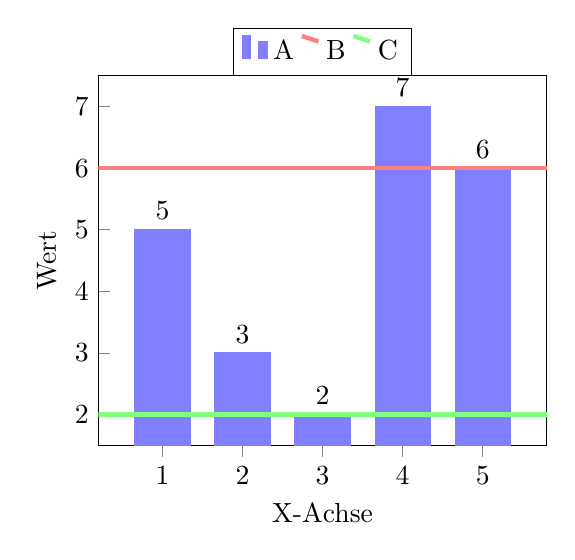
\begin{tikzpicture}
      \begin{axis}[
          xtick=data,
          ytick={0, 1, 2, 3, 4, 5, 6, 7, 8},
          x tick label style={/pgf/number format/1000 sep=},
          xlabel=X-Achse,
          ylabel=Wert,
          ytick distance=2,
          xtick pos=left,
          ytick pos=left,
          enlarge x limits=0.2,
          enlarge y limits=0.1,
          legend style={at={(0.5,1.13)},anchor=north,legend columns=-1},
          ybar,
          bar width=.7cm,
          width=0.6\textwidth,
        ]
        \addplot[
          draw=blue!50!white,
          fill=blue!50!white,
          nodes near coords,
          nodes near coords align={vertical},
        ]coordinates {(1,5) (2,3) (3,2) (4,7) (5,6)};

        \addplot[
          draw=red!50!white,
          sharp plot,
          ultra thick,
          update limits=false
        ]coordinates {(0,6) (6,6)};

        \addplot[
          draw=green!50!white,
          sharp plot,
          ultra thick,
          update limits=false
        ]coordinates {(0,2) (6,2)};

        \legend{A, B, C}

      \end{axis}
    \end{tikzpicture}
  }
  \caption{Ein Balkendiagramm}
  \label{fig:plot}
\end{figure}

\section{Quellcode-Listings}

Minted lässt inline Code wie z.B. \mintinline[style=vs]{c}{print("Hallo, LaTeX!")} zu.

Für Listings können Dateien zum Einbinden angegeben werden (Listing \ref{lst:example-file}).

\begin{listing}[!htbp]
  \inputminted{c}{./anlagen/exampleCode.c}
  \caption{C-Quelltext aus Datei}
  \label{lst:example-file}
\end{listing}

Alternativ kann der Quelltext direkt in eine \code{minted} Umgebung eingefügt werden (Listing \ref{lst:example-intext}).

\begin{listing}[!htbp]
  \begin{minted}{c}
    #include <stdio.h>

    int main(void)
    {
      printf("Hallo nochmal!\n");

      return 0;
    }
  \end{minted}
  \caption{Weiteres Beispiel für C-Quelltext}
  \label{lst:example-intext}
\end{listing}

Beide Beispiele werden im voreingestellten Stil dargestellt.
Das Paket \code{minted} bietet weitere Farbschemata, wie das Beispiel \ref{lst:example-color} zeigt.
In der Präambel des Dokuments kann mit \mintinline{tex}{\setminted{style=...}} der globale Stil der Listings angepasst werden.

\begin{listing}[!htbp]
  \renewcommand\theFancyVerbLine{%
    \rmfamily
    \textcolor[rgb]{0.7,0.7,0.7}{\tiny {\arabic{FancyVerbLine}}}%
  }
  \begin{minted}[style=solarized-dark, bgcolor=solarized@base03]{cpp}
    #include <iostream>

    int main(void)
    {
      std::cout << "Hallo (diesmal in Farbe)!" << std::endl;

      return 0;
    }
  \end{minted}
  \caption{C++ Quelltext im \textit{Solarized} Farbschema}
  \label{lst:example-color}
\end{listing}

Eine Auswahl von bereits definierten Styles ist auf der Webseite von Pygments (\url{https://pygments.org/styles/}) zu finden.

\textbf{Aber Achtung:} Die Zeilennummerierung ist standardmäßig schwarz und kann nur durch das Überschreiben von \textit{\textbackslash theFancyVerbLine} geändert werden.
Dies kann global in der Präambel (siehe \code{renewcommand...} in Listing \ref{lst:example-color}) für alle Listings geschehen oder lokal (ebenfalls Listing \ref{lst:example-color}) in der \code{listing} Umgebung.

\section{Eine Formel}

Beispiel für Formeln. Sollen Formeln linksbündig dargestellt werden, dann in der Datei \textit{header.tex} die Option \code{fleqn} entkommentieren (Option der Dokumentenklasse)\index{Formel}.

\begin{equation}
  c = \sqrt{a^2 + b^2}
\end{equation}

Im Math-Mode kann man zwar griechische Buchstaben schreiben, aber im normalen Modus nicht ohne das Paket \code{textgreek}. Aus \verb$\textmu$ wird so zum Beispiel ein \textmu.

\section{Algorithmen}

\begin{algorithm}[htb]
  \begin{algorithmic}[1]
    \REQUIRE $\Gamma$: ein Parameter \\ $M$: noch ein Parameter  \\  $m$: und noch ein Parameter \\ $k$: letzter Parameter
    \ENSURE $B = \{b_i|i = 1, 2,\dots, m\}$ ist das angestrebte Ergebnis
    \STATE Eine simple Angabe, die auch Formeln zulässt: $k$ \leftarrow $\{r_i \in \mathbb{R}^M |i = 1, 2,\dots, m\}$
    \IF{eine Zustand zutrifft}
    \STATE tue Etwas
    \ELSIF{eine Zustand zutrifft}
    \STATE tue etwas Anderes
    \ELSE
    \STATE führe die Standardaktion aus
    \ENDIF
    \FOR{$i=0$ \TO $10$}
    \STATE tue Etwas
    \ENDFOR
    \WHILE{eine Zustand zutrifft}
    \STATE tue Etwas
    \ENDWHILE
    \REPEAT
    \STATE tue Etwas
    \UNTIL{eine Zustand zutrifft}
    \LOOP
    \STATE tue Etwas
    \ENDLOOP
    \RETURN $(x+y)/2$ \COMMENT eine Anmerkung
  \end{algorithmic}
  \caption{Beispiel für einen Algorithmus}
  \label{alg:example}
\end{algorithm}

\section{Referenzen}
\label{refn}

In Kapitel \ref{beispiel} auf Seite \pageref{refn} finden Sie einige Beispiele dafür, wie Referenzen in \LaTeX~funktionieren.

\subsection{Abkürzungen}

Eine weit verbreitete Architektur für Web-Anwendungen ist der \gls{lamp}-Stack (Beispiel für die Nutzung eines Akronyms).
Wird das gleiche Akronym nochmals verwendet, wird automatisch die Kurzform \gls{lamp}-Stack verwendet.
Pluralformen sind ebenfalls automatisiert möglich, so wird aus dem \gls{qrc} im Plural die \glspl{qrc}.
Außerdem ist es möglich die volle Form, wie beim ersten Benutzen (\acrfull{qrc}), oder nur die ausgeschriebene Form (\acrlong{qrc}) zu wiederholen.

\subsection{Glossar}

MongoDB ist ein Datenbanksystem, das in die Kategorie der \gls{nosql}-Datenbanken fällt (Beispiel für einen Eintrag ins Glossar).
Manchmal wird eine Mischung aus Glossareintrag und Akronym benötigt, zum Beispiel um einen eigentlich geläufigen Fachbegriff wie \gls{dos} zu erklären.

\subsection{Symbolverzeichnis}

\begin{equation}
  \alpha = \frac{1}{e} + sin(\phi)
\end{equation}

Hier die Symbole \gls{symb:phi} und \gls{symb:e}, welche im Symbolverzeichnis erscheinen, um ihre Bedeutung zu erklären.

\subsection{Literatur}

Und natürlich kann auch auf Literatur verwiesen werden.
Alle Quellen werden in diesem Beispiel in die Datei \textit{quellen.bib} geschrieben.
In \citetitle{unterstein12} \cite{unterstein12} geht es beispielsweise um Datenbanken.
Der Artikel von \citeauthor{goldberg91} \cite{goldberg91} ist auch ganz interessant.
Zum Schluss noch eine online Quelle \cite{wave} und eine lange URL \cite{long}, die im \nameref{bib} hoffentlich ordentlich auf mehrere Zeilen aufgeteilt wird.

% \section{Ligaturtest}

% \begin{description}
%   \item[Ligaturen erlaubt]{Affe, flink, offiziell}
%   \item[Ligaturen verboten]{Kaufleute, Ablauffolge, Stoffjacke}
% \end{description}
